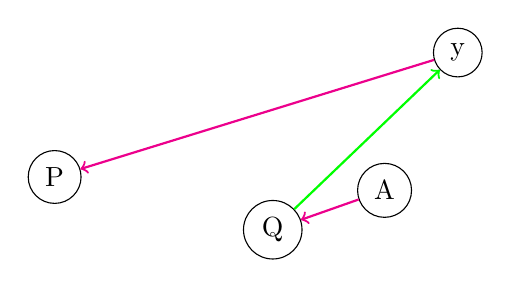
\begin{tikzpicture}
\node[circle, draw=black] (a) at (1.14, -3.86) {A};
\node[circle, draw=black] (b) at (-0.28, -4.36) {Q};
\node[circle, draw=black] (c) at (2.07, -2.11) {y};
\node[circle, draw=black] (d) at (-3.05, -3.69) {P};
\draw[->, thick, magenta] (a) -- (b);
\draw[->, thick, green] (b) -- (c);
\draw[->, thick, magenta] (c) -- (d);
\end{tikzpicture}